\documentclass[11pt, rgb]{scrreprt}
\usepackage{themeKonstanzDBIS} % Muss immer verwendet werden (Standardpaket)

\usepackage{algorithm}
\usepackage{algorithmicx}
\usepackage{algpseudocode}
\usepackage{mathtools}  % amsmath with extensions
\usepackage{amsmath} 
\usepackage{amsfonts}  % (otherwise \mathbb does nothing)
\usepackage{amssymb}  % (otherwise \mathbb does nothing)
\usepackage{nameref}
\usepackage{pgfplots}
\usepackage[normalem]{ulem}
\usepackage{array,booktabs,ragged2e}
\usepackage{pgf-umlcd}
\usepackage{wrapfig}




\format{a4}

% Thesis information        %
%\date{\today}
\year{2023}
\author{Marius Hahn}
\title{Query Processing on Dynamic Networks with Customizable Contraction Hierarchies on Neo4j}
\subtitle{thesis}
\unisection{Faculty of Sciences}
\department{Department of Computer and Information Science}
\supervisorOne{Prof. Dr. Theodoros Chondrogiannis}
\supervisorTwo{Prof. Dr. Sabine Storandt}

\headFoot{14}

%%%%%%%%%%%%%%%%%%%%%%%%%%%%%%%%%%%%%%%%%%%%%%%%%%%%%%%%%
% Begin vom Dokument                                    %
%%%%%%%%%%%%%%%%%%%%%%%%%%%%%%%%%%%%%%%%%%%%%%%%%%%%%%%%%

\begin{document}

% Thesis Title
\thesistitlepage[language=english]{MSc Thesis Title}

\chapter*{Abstract}

% Table of Contents           
\tableofcontents

%Use only if thesis is over 100 pages.
% List of figures
%\listoffigures
%\addcontentsline{toc}{chapter}{List of Figures}

%Use only if thesis is over 100 pages.
% List of tables
%\listoftables
%\addcontentsline{toc}{chapter}{List of Tables}

% For chapters and sections use  
%    \chapter{...}
%    \section{...}
%    \subsection{...}
%    \subsubsection{...}
%

\rmfamily 
\normalsize

\chapter{Introduction}

Most applications which handle data have to store these eventually.
Simple files do not offer enough semantic structure.
Therefore databases have been developed to not only store but query and aggregate data effectively and efficiently.
Relational databases that store data in tables have become the unspoken industry standard in the last decades. 
However there are domains that do not naturally fit into tables and one will need a lot of restructuring to make them fit.
As a result, there have been efforts to create databases that use other abstractions to store data, like the graph database Neo4j.

\section{Background and Motivation}

In a relational database the data is organized in tables.
Tables have rows and theses rows can be connected to other rows of the same or a different table using joins on matching cells, usually primary- foreign key relationships.
To retrieve information that is stored in two table rows one has to scan both an join them on the desired key property.
Depending on the size of the tables and the number of joins which have to be done to retrieve the desired information, such queries can be very expensive.
\\
In contrast to relational databases, graph databases treat relationships as first-class citizen.
This means a relationship that connects nodes is an entity just as the nodes it connects themselves.
As in a graph database, a node has a pointer to its relationship and a relationship has a pointer to its nodes, there is no table scan needed to retrieve connected data, which can make these queries very performant.
Such queries are shortest path queries on domains which resembles a graph by their nature, for instance road networks. 

\section{Problem and Objectives}

We focus on these shortest path queries and try to make these even quicker by employing an index call Customization Contraction Hierarchies \cite{CCH}, \textit{CCH}. 
CCH is proven to achieve a tremendous speedup compared to Dijkstra's algorithm in graphs where one can find vertices that are more important than others.
Important in this context means that these vertices belong to many shortest paths.
One example for such a domain are road networks, which we will also use in our test scenarios.

\section{Contribution}

In comparison to many other papers that examine CCH in their specific details we want to examine if we can adopt it to the graph database Neo4j, and still keep its advantages.
Will we be able to store the index in a manner which allows us to keep the performance gain we had achieved before?
Additionally we want to explore how the index behaves after updating multiple edge weights.
Will queries still be as quick as they were before the update?
This is an essential question as data in databases are usually not only stored but also manipulated.
We also want to uncover how big such an index graph will become, as there might be no need to read the index from the disk, because it easily fits in main memory.
\\
Finally we want to keep the integration into Neo4j as small as possible to make it as easy as possible at a later point to port the implementation to other graph databases that might become more relevant in future.

\chapter{Related Work} 

As this is mainly a database paper, we want to divide this chapter in two main sections \nameref{sec:algorithmic_history} and \nameref{sec:related_work:database}. \nameref{sec:algorithmic_history} 
that will give some basic overview what has been published regarding index structures to speed up shortest path queries for graphs. \nameref{sec:related_work:database} we will try 
to give an overview of efforts that have been made to make \cite[Customizable Contraction Hierarchies]{CCH} it suitable for graph databases.

\section[Algorithmic History]{Algorithmic History} \label{sec:algorithmic_history}

\cite[Contraction Hierarchies]{Geisberger_2012} or CH is heavily influenced by the idea of the \cite[Transit-Node]{Bast_2007} approach and as transit node approach itself, CCH is a
technique to speed up \cite[Dijkstras Algorithm]{Dijkstra_1959}, which is the most basic and robust algorithm to find shortest path in graphs. CH goes back to the diploma thesis of \cite[Geisberger]{Geisberger} in 2008. The \cite[Transit-Node]{Bast_2007} approach
tries to find vertices inside the graph that are more important than others. Important in this case means, these are vertices that reside on many shortest paths. This speeds up 
especially long distance queries, as one only needs to calculate the distance to the the next transit node of the source and target vertex as the shortest paths between 
the transit or access nodes will be known. \\ 
CH goes even further on the idea of having important vertices. It applies an importance to each vertex in the graph a so called rank. Furthermore it adds edges to the graph,
so called shortcuts, that preserve the shortest path property of the graph in case a vertex that is contracted resides on a shortest path between others. When querying a shortest
path CH uses a modified bidirectional-dijkstra that is restricted to only visit nodes that are of higher importance, or rank, than the its about to expand next.
This method is able to retrieve shortest paths of vertices that have a high spacial distance, however, it is rather static. In case a new edge is added or an edge weight is updated, 
it might be necessary to recontract the whole graph to preserve the shortest path property. \\
In 2016 \cite[Customization Contraction Hierarchies]{CCH} or CCH was published. The approach is the same, but in CCH shortcuts are not only added if the contraction violates the shortest path property,
they are added if there had been a connection between its neighbors through the just contracted vertex and these neighbors do not own a direct connection through an already existing edge.
The shortcut weights are later on calculated through the lowers triangle. Additionally the \cite[Customization Contraction Hierarchies]{CCH} provides an update approach that only updates,
edges that are affected by a weight change.

\section{Contraction Hierarchies Database History}\label{sec:related_work:database}

There is one bachelor thesis by Nicolai D'Effremo \cite[Some text]{DEffremo2019} that has implemented a version on \cite[Contraction Hierarchies]{Geisberger_2012} for Neo4j, one 
of the most used graph databases of today in 2023. This implementation shows that even in for databases CH is an index structure worth pursuing, as there was a tremendous speedup 
of shortest path queries paired with a reasonable preprocessing time. \cite{Zickenberg2021} showed in his bachelor thesis that it is even possible to restricted these
queries with label constraints. Although CH and CCH have little difference, sadly we could not use much of the code provided by there works. It
was deeply integrated into the Neo4j-Platform and since then two major release updates happened that have breaking changes which make it nearly impossible to reuse any of
this code.\\

Finally there is \cite[Mobile Route Planning]{Sanders} by Peter Sanders, Dominik Schultes, and Christian Vetter. In this paper it is described how one can efficiently store
the a CH index structure on a hard drive. It states an interesting technique to how store edge that are likely to be read sequentially spatially close on the hard drive which 
makes read operations that have to be done during query time fast. The motivation of \cite[Mobile Route Planning]{Sanders} through was slightly different. They came up with this
idea because computation power on mobile devices is limited, so they could precalculate the CH index on a server and then later distribute it to a mobile device.
\\
We will use parts of this idea and partly port it to our database context as we suppose there are many similarities.

\chapter{Preliminary}

As the target platform for this work is the graph database neo4J, we will mostly consider \textit{directed} graphs. From the terminology we always refer \textit{arcs}, which is an directed edge.
In some rare cases we might refer to \textit{edges}. There you can be sure that it doesn't matter weather it is directed or not.

\section{Notation and Expressions}
We denote a graph $G(V, A)$ in case me mean an \textit{directed} graph, where $v$ is a vertex contained in the vertices $v \epsilon  V$ and $e$ is an
edge $a \epsilon A$. An arc is uniquely defined by to vertices $v_a$ and $v_b$ such that $v_a \neq v_b$, so there are no loops nor multi edges.
An edge additionally has a weight function $w: E \rightarrow \mathbb{R}_{<0} $ it's weight which must be a positive.
\\
$G$ represents the input graph. The contraction graph $G'(V', A')$ is the graph that will be used at contraction for initially building the CCH index structure. A vertex $v$ in will 
never be really deleted. Instead the rank property $r(v)$ is set to mark this as an already contracted. So $V \equiv V'$ but $A \subseteq A'$ there will be edges add while building
the CCH index. $S = A' \setminus A$ is the shortcut set that is added throughout the contraction. 
\\
$G^*(V^*, A^*)$ is the is the search graph while doing one a shortest path query. Futhermore one query will have two search graphs. $G^*_\uparrow$ representing the upwards search graph
and the $G^*_\downarrow$.
\\
Finally there will be the edge set of edges that are written to the disk. These will $\bigcirc E$ will be separated into to sets $\bigcirc E_\downarrow$ and $\bigcirc E_\uparrow $, too.


\section{Customizable Contraction Hierarchies}\label{sec:Preliminary_CCH}


\chapter{Customizable Contraction Hierarchies}\label{sec:Preliminary_CCH}

In this section we will present the basic idea of \cite[Customization Contraction Hierarchies]{CCH} and also work out the main difference between CCH and \cite[Contraction Hierarchies]{Geisberger_2012}.
It is far form being complete, but there will be some easy examples to show the concept. 

\section{Contracting and Searching}

\begin{figure}
    \centering
    \input{assets/tikz/contractingAndSeaching.tex}
    \caption{The numbers inside the vertices represent their contraction order}
    \label{fig:contrating_and_searching}
\end{figure}

In Figure \ref{fig:contrating_and_searching} you can see a contracted graph $G(V,E')$. The solid lines represent the original edges $E$ of a graph $G$. The dashed lines between vertices are shortcuts $S$ that 
have been added while creating the CCH index graph G'(V, E'). The numbers inside the vertices reflect the contraction order.
\\
Contracting a vertex means deleting it. While contracting a vertex we want to preserve its via connection. If a vertex that is contracted resides on a simple path between two vertices of higher rank,
and there is no edge $e \epsilon E'$ between these vertices a shortcut has to be inserted between the two. 
Let's reconstruct the contraction of Figure \ref{fig:contrating_and_searching}. At first vertex $v(1)$ is removed. As $v(1)$ resides on a simple path to between $v(3)$ and $v(5)$ and there is no edge $e(v(3), v(5)) \notin E'$,
there must be a shortcut insert to keep the via path.
The same applies after contracting $v(2)$ for the vertices $v(4)$ and $v(5)$. For all the other vertices we do not need to insert shortcuts.
\\
As we preserved all via paths during the contraction the shortest path can be retrieved by a bidirectional Dijkstra that is restricted such that it only expands vertices of higher rank. 
Note that the target side walks the in counter direction. 
Therefore if one wants to retrieve the shortest path between $v(3)$ and $v(4)$ there will be a forward search from $v(3)$ and a backward search from $v(4)$. As we restrict theses searches to expand only vertices
of higher rank, the only vertex to expand is $v(5)$ for both searches which is is a meeting point, too. Finding at least one meeting point in the forward an backward search means there exist a path between them.
After merging these paths at the middle vertex $v(5)$ one will obtain the shortest path.
\\
For an arbitrary contracted graph is it possible that there are more than one meeting point. As merging two shortest paths will not necessary lead to an other shortest path, one has to merge
all possible meeting points and take the path among the merged ones which has the smallest distance. 
\\ 
The stopping condition for such a CH-Search is either, both forward and backward search, have reached the top node so there is no further vertex to expand, which happens in the example of figure \ref{fig:contrating_and_searching} or, backward and forward search exceed to 
the length that has already been found among the merged paths.

\section{Difference between CH and CCH}

Looking at the left graph in Figure \ref*{fig:DifferenceCHAndCCH} it has been contracted in the CH way, whereas the right is the CCH way. We explicitly state this here because 
we have found paper \cite{Ouyang_2020} that mix up these well known names, claiming they to Contraction Hierarchies CH while actually doing Customizable Contraction Hierarchies CCH. 
The main difference is, CH will only insert an shortcut between two nodes if the node that is contracted resides on the shortest path between two of its neighbors. 
When vertex $v(1)$ is contracted there is no shortcut inserted as vertex $v(1)$ is not on the shortest path between which is via vertex $v(4)$.
\\
whereas in the CCH case the edge weights do not play a role a contraction time. If a node is contracted and there is no direct connection between two of its neighbors, one has to insert a shortcut. This gives
the advantage that later on we can easily update edge weights without inserting new shortcut, as all possibly needed shortcuts already exist.
\\ 
Let's complete this example by updating the edge $e(v(2), v(4))$ that currently has the weight of $w(e)=1$ to $w(e) = 5$. Now the vertex $v(1)$ is on the shortest path between vertex $v(2)$ and $v(3)$. 
To update the CH graph we have to insert an edge between vertex $v(2)$ and $v(3)$ whereas the topological structure of the CCH remains the same, one only need to update the weight and the middle node of the already give shortcut.

\begin{figure}
    \centering
    \input{assets/tikz/DifferenceCHAndCCH.tex}
    \caption{The left represents a CH and the right a CCH contracted graph}
    \label{fig:DifferenceCHAndCCH}
\end{figure}

\section{Metric Dependent Vertex Order}
There are two ways to get a suitable vertex order. A so called \textit{metric independent} and a so called \textit{metric dependent} one. The metric independent recursively uses balanced separator to determine a vertex ordering\cite{CCH}. Although this is the superior method, it is not used in this paper writing an algorithm that calculates balanced separators isn't trivial, and we are not aiming for optimizing the contraction process. 
The metric dependent order mainly uses the edge difference $ED$ to determine which vertex is to be contracted next. The $ED$ is determined as the $|edges To Insert| - |edges To Remove|$. The fewer edges are inserted during contraction the fewer edges will be contained by the final graph, therefore fewer edges to expand in a search. However using only the edge differences doesn't lead to desired result. This is because during contraction there will be areas that get less dense than others. 
There are two problems that can arise. One is that important vertices are not contracted last. The other is the search space of the query gets linear although it could be logarithmic.

\subsection{Important Vertices not contracted last}\label{sec:not_contracted_last}

\begin{figure}
    \centering
    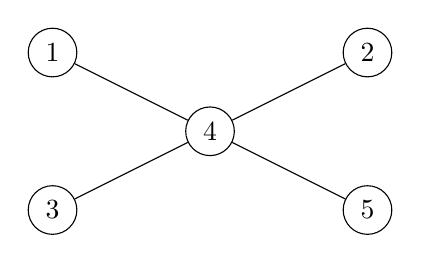
\begin{tikzpicture}[node distance={15mm}, main/.style = {draw, circle}]
    \node[main] (x1) at (1, 2) {$1$}; 
    \node[main] (x3) at (1, 0) {$3$};
    
    \node[main] (x4) at (3, 1) {$4$}; 
    
    \node[main] (x2) at (5, 2) {$2$}; 
    \node[main] (x5) at (5, 0) {$5$}; 
    
    \draw (x1) -- (x4);
    \draw (x2) -- (x4);
    \draw (x3) -- (x4);
    \draw (x5) -- (x4);
    
\end{tikzpicture} 
    
    \caption{The numbers inside the vertices represent their contraction order}
    \label{fig:not_contracted_last}
\end{figure}

Looking at figure \ref{fig:not_contracted_last}, this is a possible contraction order, if only the $ED$ is used to contract vertices. At the beginning the nodes with rank 1, 2, 3, 5 have the same edge difference, which is $ED = -1$. One edge after another will be removed after contraction and the is no shortcut inserted. This happens until there are only the vertices 4 and 5 left. Now vertex 4 has an $ED=-1$, too, same as vertex 5. Therefore the algorithm contracts the vertex with rank 4 before the one with rank 5. \\
However this is not the desired result. There are six ${(1,2), (1,3), (1,5), (2,3), (2,5), (3,5)}$ shortest paths that involve vertex 4, all the other vertices do not encode any shortest path, so vertex 4 should be contracted last. The search graph on the right of Figure \ref{fig:not_contracted_last} shows why. Imagine we we do a shortest path query between $v(1)$ and $v(3)$. After expanding both, the forward and the backward search, to $v(4)$ there is yet another vertex we'll have to expand $v(5)$, although 
as you can see in the original graph on the right, its not possible that $v(5)$ is on the shortest path. Therefore a better contraction order would be a in Figure \ref{fig:contrating_and_searching}.  This can be overcome by the method that is explained in section \ref{sec:vertex_importance}.

\subsection{Linear Query Search Space}\label{sec:linear_query}

\begin{figure}
\centering
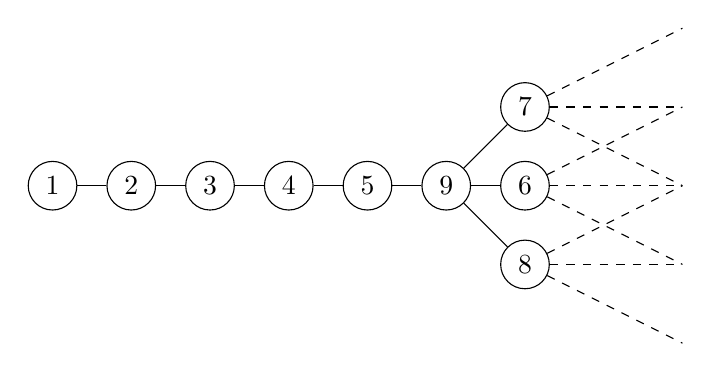
\begin{tikzpicture}[node distance={15mm}, main/.style = {draw, circle}]

    \node[main] (x1) at (0, 0) {$1$};
    \node[main] (x2) at (1, 0) {$2$};
    \node[main] (x3) at (2, 0) {$3$};
    \node[main] (x4) at (3, 0) {$4$};
    \node[main] (x5) at (4, 0) {$5$};
    \node[main] (x9) at (5, 0) {$9$};
    
    \node[main] (x7) at (6, 1) {$7$};
    \node[main] (x8) at (6, -1) {$8$};
    \node[main] (x6) at (6, 0) {$6$};
    
    
    \draw (x1) -- (x2);
    \draw (x2) -- (x3);
    \draw (x3) -- (x4);
    \draw (x4) -- (x5);
    \draw (x5) -- (x9);
    
    \draw (x6) -- (x9);
    \draw (x9) -- (x7);
    \draw (x9) -- (x8);
    
    \draw [dashed] (x7) -- (8, 2);
    \draw [dashed] (x7) -- (8, 1);
    \draw [dashed] (x7) -- (8, 0);
    
    \draw [dashed] (x8) -- (8, 0);
    \draw [dashed] (x8) -- (8, -2);
    \draw [dashed] (x8) -- (8, -1);
    
    \draw [dashed] (x6) -- (8, 1);
    \draw [dashed] (x6) -- (8, 0);
    \draw [dashed] (x6) -- (8, -1);
    
\end{tikzpicture} 
    
\caption{Linear Contraction}
\label{fig:linear_contraction}
\end{figure}

Regarding figure \ref{fig:linear_contraction} there are three possible index graphs $G'$ of one and the same base graph $G$. The numbers inside the vertices represent the contraction order.
\\
The first one could be contracted using the edge difference $ED$, as always one of the outer vertices with $ED=-1$ was contracted. On the one hand it reaches the optimum in case for textit{least shortcuts inserted}. On the other though it has the worst search space among the three vertex orderings. 
To get from node $v(1)$ to $v(5)$ we have to expand four vertices. 
\\
The second $G'$ one contracts the middle vertices, which encodes the most shortest paths, first and therefore inserts three shortcuts. Although this example has a lot of shortcuts, there are still a lot of vertices to expand in some cases. In case every node of $G$ has a weight of $1$, and one wants to go from $v(1)$ to $v(5)$ the forward search will have to expand four nodes as in the upper first example.
\\
The third example contracts the middle node last. At first it contracts the nodes right next to the middle node. Therefore we have to insert shortcuts between $e(v(3)v(5))$ and $e(v(4), v(5))$.
Therefore no matter what source, target pair we are trying to find in this example, the forward and the backward search will have to expand at most one single node. This example additionally shows that
recursively finding a balanced separator, as proposed in \cite[Customization Contraction Hierarchies]{CCH}, is very a promising method to obtain a good contraction order. Sadly there was no time to 
investigate any further in this direction.  

\section{Vertex importance}\label{sec:vertex_importance}

As shown in section \ref{sec:not_contracted_last} and \ref{sec:linear_query} using only the $ED$ as a metric to determine which vertex to contract next is not sufficient to get a suitable

\section{Perfect Customization}

\begin{figure}
    \centering
    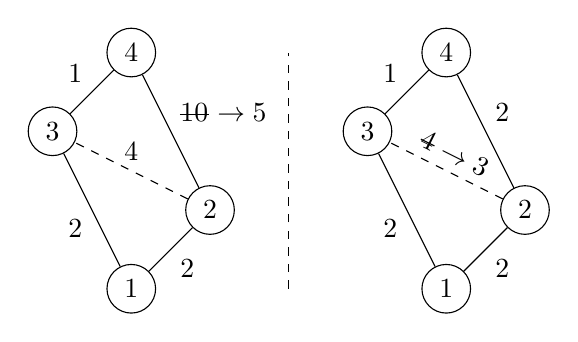
\begin{tikzpicture}[node distance={15mm}, main/.style = {draw, circle}]

    \node[main] (x3) at (0, 2) {$3$};
    \node[main] (x4) at (1, 3) {$4$};
    \node[main] (x2) at (2, 1) {$2$};
    \node[main] (x1) at (1, 0) {$1$};
    
    \draw (x1) -- node[below right] {$2$}(x2);
    \draw (x1) -- node[below left] {$2$} (x3);
    \draw (x2) -- node[above right] {\sout{$10$} $\rightarrow 5$} (x4);
    \draw (x3) -- node[above left] {$1$} (x4);
    \draw[dashed] (x2) -- node[above] {$4$} (x3);

    \draw[dashed]  (3,0) -- (3,3);

    \node[main] (x31) at (4, 2) {$3$};
    \node[main] (x41) at (5, 3) {$4$};
    \node[main] (x21) at (6, 1) {$2$};
    \node[main] (x11) at (5, 0) {$1$};
    
    \draw (x11) -- node[below right] {$2$}(x21);
    \draw (x11) -- node[below left] {$2$} (x31);
    \draw (x21) -- node[above right] {$2$} (x41);
    \draw (x31) -- node[above left] {$1$} (x41);
    \draw[dashed] (x21) -- node[above, sloped] {\sout{$4$} $\rightarrow 3$}  (x31);

    
\end{tikzpicture}
    \caption{Disk Block}
    \label{fig:perfectCustomization}
\end{figure}

Here is an example why perfect customization is necessary to get the full
benefit of CCH.

\chapter{Integration in a Neo4j}

In this section it is described how "Customizable Contraction Hierarchies" CCH is integrated into Neo4j. CCH arguments the input graph, which means it inserts arcs, so called shortcuts, that do not belong to the original data. To keep the change to the input graphs as little as possible we decided to not insert any arc into the graph that is stored inside the neo4j database, but introduce another graph data structure, the index graph. This index graph has an mapping to the input graph that is held by the database, by inserting two properties into the node of the input graph. The \textit{rank} this vertex has in the index graph and the \textit{indexing weight} it had during the last customization process. This gives yet another two advantages. One is that we get full control about the graph representation which is helpful to efficiently store and read the index graph for the disk. Another is that the with this approach it makes it easier to later on port the idea to another graph database manufactures.

\section{Index Graph Data Structure}\label{sec:index_graph}

The index graph data structure is neither a adjacency list nor adjacency matrix. There is a vertex object that has two hash tables. One for incoming arc and one for outgoing arcs. The hash tables keys are of type vertex and the value is the arc. An arc has a reference to its start vertex and one to its end vertex. \\
A disadvantage of this model could be that some modern hardware optimization that exist for arrays do not match with this data structure. When using an array, the values this array are stored sequentially in main memory. When one value of an array is accessed by the CPU, modern hardware reads subsequent values into the CPU-cache because it is likely that they are accessed right after it. The model of the index graph is a linked data structure, a bit like a linked list. The elements of an linked list are contained somewhere in main memory. There is no guarantee that subsequent values have any spacial proximity. Therefore the just explained hardware optimization will not give any advantage. \\ % cite some paper to this topic
However, this makes the makes the graph traversal easy. Additional it makes it very efficient to explore the neighborhood of a vertex. There is no array traversal to find a vertex and only one hash table lookup for finding an arc of a vertex. Additionally these hash tables only contain few elements. This makes this data structure efficient anyway. Test on small graphs [Oldenburg] show that cch queries can be answered in less than one millisecond, which is close to what we tested with the original cch application.

\section{The Mapping}\label{sec:mapping}

The in memory data structure of neo4j is similar to the just explained index graph data structure in section \ref{sec:index_graph}. A \textit{node} has a collection of \textit{relationships} and a \textit{relationship} has a reference to its \textit{start node} and \textit{end node}.
As neo4j is a full blown property graph nodes and relationship contain a lot of other information. A node has a collection of \textit{labels}, relationship has a \textit{type}. The class \textit{Node} and the class \textit{Relationship} 
are both derived from the class \textit{Entity} which also has a collection of properties as well as and id that is managed by the database system. Note that, as of version Neo4j 5.X, this id can change over time and should not be used to make mappings to external systems. Additionally 
worth to mentioning here is that the Neo4j system shifted its id concept as it moved from major release 4 to 5. Until major release 4 every entity had a unique integer identifier. Since major release 5 every entity has a string identifier which is a UUID and the old \textit{id} identifier
isn't guaranteed to be unique anymore. It is deprecated and marked for removal.
\\
As just explained there are lot of information in this data structure. A lot of information we don't need. Looking at \ref{fig:mapping} we only want to keep track of the information that is needed for the CCH index. Additionally as disks are
divided  into blocks and sectors we want to flatten the graph which is in memory more looks like a tree to a structure that looks like a table. Therefore we decided that the disk data structure only consists of edges $\bigcirc A$. A disk edge $a \epsilon \bigcirc A$ consists of four values, 
the \textit{start rank}, the \textit{end rank}, the \textit{start rank} and the \textit{weight} . The middle node is set $-1$ in case that this arc, is an arc of the input graph. We will get two edge sets $\bigcirc A_\downarrow$ for the downwards graph and $\bigcirc A_\uparrow $ upwards graph.
$\bigcirc A_\downarrow$ contains all downward edge that which are needed for the backward search and $\bigcirc A_\uparrow$ contains all upwards arcs that are needed for the forward search.
\\
During the the contraction every node gets a rank assigned. This rank is the only change that is made to the Neo4j data structure and its the mapping identifier between the input graph $G$ and the index graph $G'$. $G'$ will then be used to generate $\bigcirc A_\downarrow$ and $\bigcirc A_\uparrow$.


\begin{figure}
    \centering
    \begin{tikzpicture}[node distance={15mm}, main/.style = {draw, circle}]
 
    \node[main, align=center] (x3) at (0,4) {id:23, labels:\{\\Location,…\}, \\props:\{\\rank:3,…\}};
    \node[main, align=center] (x2) at (12,2) {id:22, labels:\{\\Location,…\}, \\ props:\{\\rank:2,…\}};
    \node[main, align=center] (x1) at (6, 0) {id:21, labels:\{\\Location,…\},  \\ props:\{\\rank:1,…\}};
    
    \draw[ -Stealth] (x2) -- node[rectangle,draw, fill=white,  align=center] {:ROAD \\ weight:1.0}(x1);
    \draw[ -Stealth] (x1) -- node[rectangle,draw, fill=white,  align=center] {:ROAD \\ weight:1.0} (x3);
    \draw[dashed, -Stealth] (x2) -- (x3);

    \draw (0,-2) -- (10,-2);
    \draw (0,-2.5) -- (10,-2.5);
    \draw (0,-3) -- (10,-3);
    \draw (0,-3.5) -- (10,-3.5);
    \draw (0,-4) -- (10,-4);

    \draw (0,-2) -- (0,-4);
    \draw (2.5,-2) -- (2.5,-4);
    \draw (5,-2) -- (5,-4);
    \draw (7.5,-2) -- (7.5,-4);
    \draw (10,-2) -- (10,-4);

    \node[align=center] at (1.25, -2.25) {\textbf{start rank}};
    \node[align=center] at (3.75, -2.25) {\textbf{end rank}};
    \node[align=center] at (6.25, -2.25) {\textbf{middle rank}};
    \node[align=center] at (8.75, -2.25) {\textbf{weight}};

    \node[align=center] at (1.25, -2.75) {2};
    \node[align=center] at (3.75, -2.75) {3};
    \node[align=center] at (6.25, -2.75) {1};
    \node[align=center] at (8.75, -2.75) {2.0};

    \node[align=center] at (1.25, -3.25) {1};
    \node[align=center] at (3.75, -3.25) {3};
    \node[align=center] at (6.25, -3.25) {-1};
    \node[align=center] at (8.75, -3.25) {1.0};

    \node[align=center] at (1.25, -3.75) {2};
    \node[align=center] at (3.75, -3.75) {1};
    \node[align=center] at (6.25, -3.75) {-1};
    \node[align=center] at (8.75, -3.75) {1.0};

\end{tikzpicture}
    \caption{mapping}
    \label{fig:mapping}
\end{figure}

\section{How to Store the Index Graph}

After generating the disk arc sets $\bigcirc A_\downarrow$ and $\bigcirc A_\uparrow$, we now want to store them as efficiently as possible to the disk. To refine the definition of a disk arc. It consist of four values \textit{start rank}, the \textit{end rank}, the \textit{start rank} and the \textit{weight}. The
first three are 32 bit signed integer, which gives a maximum indexable amount of vertices for $2^{16}$. The last one, the arc \textit{weight} is a 32 bit floating point number. One could argue that 32 bit are not very precise, though our experiments we never had any imprecision problem. Furthermore, little imprecision
would not cause a big problem, as the index graph is only needed to find the shortest path. The exact weight can later on be retrieved after the shortest path is resolved in $G$. 
\\
This 16 Byte disk collected to disk blocks, that have at least the size of one disk block on the systems hard drive, as usually the system will always read a complete disk block even if you request only 16 Byte of information. But it is possible to make blocks bigger than one disk block. This can be wanted if you have a big read cache,
or even need it the highest outgoing or in ingoing arc degree exceed the $\frac{diskBlockSize}{16}$ as you will see in \ref{sec:persistanceOrder}.

\begin{figure}
    \centering
    \begin{tikzpicture}[node distance={15mm}, main/.style = {draw, circle}]
    
    \draw (-7,6) rectangle (-1,7);
    \draw (-5.5,6) -- (-5.5,7);
    \draw (-4,6) -- (-4,7);
    \draw (-2.5,6) -- (-2.5,7);
    \node at (-6.25, 6.5) {from};
    \node at (-4.75, 6.5) {to};
    \node at (-3.25, 6.5) {middle};
    \node at (-1.75, 6.5) {weight};

    \draw [decorate,decoration = {brace, amplitude=5pt}] (-7,7.1) --  (-5.5,7.1);
    \draw [decorate,decoration = {brace, amplitude=5pt}] (-5.5,7.1) --  (-4,7.1);
    \draw [decorate,decoration = {brace, amplitude=5pt}] (-4,7.1) --  (-2.5,7.1);
    \draw [decorate,decoration = {brace, amplitude=5pt}] (-2.5,7.1) --  (-1,7.1);
    \node[ align=center] at (-6.25, 7.8) {32 bit  \\ integer};
    \node[ align=center] at (-4.75, 7.8) {32 bit  \\ integer};
    \node[ align=center] at (-3.25, 7.8) {32 bit  \\ integer};
    \node[ align=center] at (-1.75, 7.8) {32b bit \\ integer};

    \draw [decorate,decoration = {brace, amplitude=5pt}] (-1,5.9) --  (-7, 5.9);
    \node at (-4, 5.5) {16 byte DiskArc};

    \draw[dashed, -Stealth] (-1,7) -- (0, 6.7);
    \draw[dashed, -Stealth] (-1,6) -- (0, 6.3);
    
    
    \draw (0,7) -- (4,7);
    \draw[dashed] (0,6) -- (4,6);
    \draw[dashed] (0,5) -- (4,5);
    \node at (4.5,5) {0};
    \node at (4.5,1) {1};
    \draw (0,3) -- (5,3); 
    \draw[dashed] (0,2) -- (4,2);
    \draw[dashed] (0,1) -- (4,1);
    \draw[out=60, in=-120] (0,0) to (4, 0);
    \draw (0,0) -- (0,7); 
    \draw (4,0) -- (4,7); 
    \node at (2, 6.5) {DiskArc};
    \node at (2, 5.5) {DiskArc};
    \node[rotate=90, font=\Large] at (2, 4) {. . . . .};
    
    \node[rotate=-90] at (5.85, 5) {disk block};
    \draw [decorate,decoration = {brace, amplitude=10pt}] (5.2,7) --  (5.2,3);

    \node at (2, 7.2) {\textbf{Arc File}};

    %---------------------------------------------------------
    \draw (-7,0+1.5) -- (-1,0+1.5);
    \draw (-7,1+1.5) -- (-1,1+1.5);
    \draw (-7,-0.5+1.5) -- (-7,1+1.5);
    \draw (-5.5,-0.5+1.5) -- (-5.5,1+1.5);
    \draw (-4,-0.5+1.5) -- (-4,1+1.5);
    \draw (-2.5,-0.5+1.5) -- (-2.5,1+1.5);
    \draw[out=60, in=-120] (-1,0+1.5) to (-1,1+1.5);

    \node at (-6.25, 0.5+1.5) {37};
    \node at (-4.75, 0.5+1.5) {293};
    \node at (-3.25, 0.5+1.5) {73};
    \node at (-1.75, 0.5+1.5) {…};

    \node at (-8.5, 0.5+1.5) {disk block:};
    \node at (-8.5, -1+1.5) {rank:};
    \node at (-7, -1+1.5) {0};
    \node at (1.5-7, -1+1.5) {1};
    \node at (3-7, -1+1.5) {2};
    \node at (4.5-7, -1+1.5) {3};

    \draw [decorate,decoration = {brace, amplitude=5pt}] (-7,1.1+1.5) --  (1.5-7,1.1+1.5);
    \node[ align=center] at (0.75-7, 1.8+1.5) {32 bit  \\ integer};
    \node[ align=center] at (-4, 1.2+1.5) {\textbf{Position File}};
\end{tikzpicture}
    \caption{Disk Block}
    \label{fig:disk_block}
\end{figure}

\subsection{Persistance Order}\label{sec:persistanceOrder}

As the disk arc are later on is used for the CCH search, we want to sequentially write them in a way that provides a high spatial proximity of vertices that are likely to get requested together. Here we will adopt the idea of \cite[Mobile Route Planning]{Sanders}. In the transformation form $G'$ to its disk arcs $\bigcirc A_\uparrow$ 
and $\bigcirc A_\downarrow$ we do a simple depth first search on all ingoing arcs on the target rank to determine the order for $\bigcirc A_\uparrow$. We do the same for all outgoing arcs on the source rank to determine the order for $\bigcirc A_\downarrow$.
There is one file for storing all upward arc and on file storing all downward arcs. Each of this files has a position file that belongs to it, as shown in figure \ref{fig:position_file}. After every vertex that is expanded, all its arcs are pushed to a buffer of size disk block. If the buffer is full or the number of arcs doesn't fit anymore,
the buffer is flushed to the current position in the arc file and the file position is incremented by $1$. The store position is saved in the position file of the arc file, such that we can find the arcs back later on. If the buffer wasn't complete full all remaining arc slots are filled with dummy arcs that contain only $-1$ at every property.


\begin{figure}
    \centering
    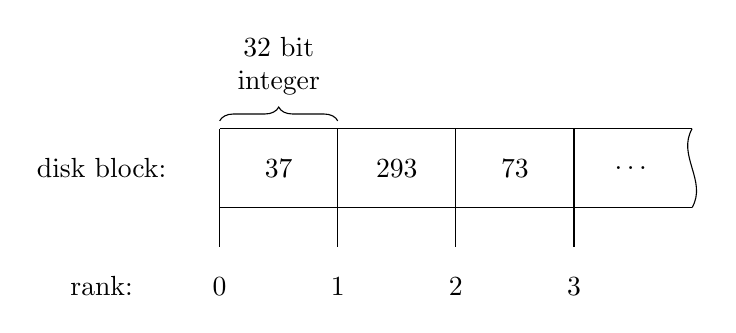
\begin{tikzpicture}[node distance={15mm}, main/.style = {draw, circle}]

    \draw (0,0) -- (6,0);
    \draw (0,1) -- (6,1);
    \draw (0,-0.5) -- (0,1);
    \draw (1.5,-0.5) -- (1.5,1);
    \draw (3,-0.5) -- (3,1);
    \draw (4.5,-0.5) -- (4.5,1);
    \draw[out=60, in=-120] (6,0) to (6,1);

    \node at (0.75, 0.5) {37};
    \node at (2.25, 0.5) {293};
    \node at (3.75, 0.5) {73};
    \node at (5.25, 0.5) {…};

    \node at (-1.5, 0.5) {disk block:};
    \node at (-1.5, -1) {rank:};
    \node at (0, -1) {0};
    \node at (1.5, -1) {1};
    \node at (3, -1) {2};
    \node at (4.5, -1) {3};

    \draw [decorate,decoration = {brace, amplitude=5pt}] (0,1.1) --  (1.5,1.1);
    \node[ align=center] at (0.75, 1.8) {32 bit  \\ integer};

\end{tikzpicture}
    \caption{Position File}
    \label{fig:position_file}
\end{figure}

\section{Reading Disk Arcs}

If one wants to get all upwards arcs of rank $i$ one need take  the upwards position file, retrieve the integer $j$ that is stored at index $i$, and then read the complete block $j$ in the upwards arc file. There
There one will get an array, contain the requested arcs but also some other. These arcs are likely to be request next. Therefore we want to keep them in memory. We implemented two buffer a \textit{circular buffer} and a \textit{least recently used buffer} LRU

\subsection{Circular Buffer}

For the circular buffer we simply used an array of disk arcs. If we reach the end of the buffer we restart overwriting the values from the array start. To get the all arcs of a rank one request that rank number. There is a position hash table which tells the start position of that rank inside the buffer. If it is missing, the containing disk block is read to the buffer. It 
continues to read sequentially until the request rank and the read arc doesn't belong together anymore. This buffer has the advantage that we can exactly determine the amount of arcs we buffering. Also as it is just a simple array, it will be easy for the operation system to cache it.
The disadvantage is that it is possible that we request arc sets very often as it is possible they get evicted just before request again.

\subsection{Least Recently Used Buffer}

Cache is a \textit{java.util.LinkedHashMap}. This class provides the possibility to evicted the entry that has been requested longest time ago. In our case it maps ranks to sets of disk arcs. We can only determine how many 
disk arc sets we have in memory and disk arc sets do not have always the same size. Higher rank vertex usually have bigger sets as they are of higher degree. The advantage is, it is very easy to implement and therefore very 
resilient to programming errors.

\section{The Search}

The search brings all things explained in this chapter together. 

%\begin{figure}
%    \centering
%    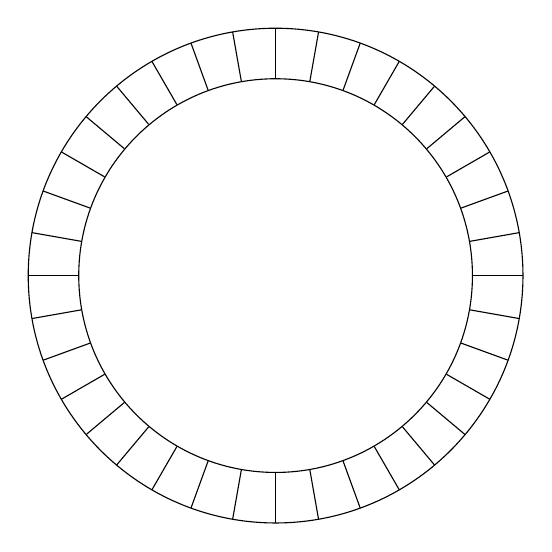
\begin{tikzpicture}[node distance={15mm}, main/.style = {draw, circle}]

    \draw (0,0) node[main, minimum size=5cm](z0) {} circle (pi);
    \draw (z0) -- (10:pi) node[midway,above]{};
    \draw (z0) -- (20:pi) node[midway,above]{};
    \draw (z0) -- (30:pi) node[midway,above]{};
    \draw (z0) -- (40:pi) node[midway,above]{};
    \draw (z0) -- (50:pi) node[midway,above]{};
    \draw (z0) -- (60:pi) node[midway,above]{};
    \draw (z0) -- (70:pi) node[midway,above]{};
    \draw (z0) -- (80:pi) node[midway,above]{};
    \draw (z0) -- (90:pi) node[midway,above]{};
    \draw (z0) -- (100:pi) node[midway,above]{};
    \draw (z0) -- (110:pi) node[midway,above]{};
    \draw (z0) -- (120:pi) node[midway,above]{};
    \draw (z0) -- (130:pi) node[midway,above]{};
    \draw (z0) -- (140:pi) node[midway,above]{};
    \draw (z0) -- (150:pi) node[midway,above]{};
    \draw (z0) -- (160:pi) node[midway,above]{};
    \draw (z0) -- (170:pi) node[midway,above]{};
    \draw (z0) -- (180:pi) node[midway,above]{};
    \draw (z0) -- (190:pi) node[midway,above]{};
    \draw (z0) -- (200:pi) node[midway,above]{};
    \draw (z0) -- (210:pi) node[midway,above]{};
    \draw (z0) -- (220:pi) node[midway,above]{};
    \draw (z0) -- (230:pi) node[midway,above]{};
    \draw (z0) -- (240:pi) node[midway,above]{};
    \draw (z0) -- (250:pi) node[midway,above]{};
    \draw (z0) -- (260:pi) node[midway,above]{};
    \draw (z0) -- (270:pi) node[midway,above]{};
    \draw (z0) -- (280:pi) node[midway,above]{};
    \draw (z0) -- (290:pi) node[midway,above]{};
    \draw (z0) -- (300:pi) node[midway,above]{};
    \draw (z0) -- (310:pi) node[midway,above]{};
    \draw (z0) -- (320:pi) node[midway,above]{};
    \draw (z0) -- (330:pi) node[midway,above]{};
    \draw (z0) -- (340:pi) node[midway,above]{};
    \draw (z0) -- (350:pi) node[midway,above]{};
    \draw (z0) -- (0:pi) node[midway,above]{};
    
\end{tikzpicture}
%    \caption{Circular Buffer}
%    \label{fig:circular_buffer}
%\end{figure}

\chapter{Experiments}

In this chapter we will experimentally check if our idea and implementation of a persisted version of CCH works out. We will give an answer to the following Questions:
\begin{itemize}
    \item What is the largest graph we are able to index?
    \item Are we able to beat dijkstra's performance? if yes, by how much?
    \item Is there a category of queries that work better than others?
    \item Do different buffer sizes significantly change the performance?
    \item Is the input graph size the only factor that affect the performance?
    \item How long do updates take if we change all arc weights?
    \item Do updates effect performance of the search?
\end{itemize}

\section{The Test Environment}

We implemented this CCH in \textit{Java 17} and fo \textit{Neo4j 5.1.0}. The only addition Java library we use is \textit{lombok version 1.18.24}, for static code generation, like getter and setters.
\\
The code runs on a virtual machine that is running \textit{Linux Mint 20.3 Una}. This VM has two  AMD EPYC 7351 16-Core Processors with L1d cache=1 MiB L1i cache=2 MB, L2 cache=16 MB and L3 cache=128 MB. 
It has 512 GB of RAM and the system hard drive is a \textit{Intel SSDPEKNW020T8} SSD with 2 TB.
The fact that our test environment uses a SDD hard drive isn't ideal. Databases usually use HDD drives which are slower in reading data but faster in writing data. However, a quick lookup on the internet shows that,
as of today, in November 2023, HDD drives start at a price of around 15€/TB and have 512MB of cache. Our biggest index has 430MB in total, depending on the caching algorithm of the disk, it could be that 
the HDD would pre cache the whole index anyway, such that there are fewer actual reads from the durning disks in the HDD and the read performance gets closer to what a SSD can achieve.

\section{The Test Data}

The test graphs we evaluate the implementation are provided by the \cite[9th DIMACS Implementation Challenge - Shortest Paths]{DIMACS}. There we focus on the road networks of New York, Colorado, Florida, California+Nevada and also larger networks that represent the great lakes on the north american continent as well as the USA east cost.
We use the distance graphs, only in case of New York we tried the distance and the time travel graph. As the results were similar and the contraction strategy is not depending on the arc weight we omitted the further test wit the time travel graphs.
The arc size differs from the DIMACS Challenge as we have filtered out duplicate edges.

\section{The Contraction}

In table \ref{tab:overview_table} you can see the basic results of the networks we tested. One would think that the contraction time goes along with the size of the network, though it doesn't. The New York graph has has about the same contraction time 
as Florida which is about three times as big. Additionally the amount of shortcuts inserted Relative to the already existing arcs is almost twice as big. This is probably happens because the New York graph is a lot denser than the other graphs under test like Florida.
In New York, regardless if you take the state or only the city itself, there are four natural separators: \textit{Manhattan and Brooklyn}, \textit{Manhattan and Queens}, \textit{Manhattan and Bronx}, \textit{Bronx and Queens}, \textit{Staten Island and Brooklyn} as well as \textit{Staten Island and Manhattan to the mainland}.  
\\ 
Where as the population of Florida is more sparse and located on a line at the cost of both side, as well as their streets. Therefore as shown in figure \ref{fig:linear_contraction} the contraction can easily find vertices as separators. 

\subsection{Limits} \label{sec:contraction_limits}

We decided to set the time limit a contraction should not exceed to about one day. If, within this time the contraction did finish, we decided to abort the process. This happend for the graphs \textit{Western USA}, therefore we didn't try larger ones. If one would want to go this size or bigger we suggest,
to achieve the vertex ordering by recursive finding balanced separators as described in \cite[Customization Contraction Hierarchies]{CCH}. 
\\
Contraction methods that rely on measures like edge difference suffer from very bad performance, if the graph gets dense. At the same time, the remaining graph will get denser towards the end of the contraction process. It is possible  that the last few nodes form a complete graph. The graph that \textit{Great Lake} turned complete with $1078$ nodes left in the queue. 
at this time it toke about 110 second to contract a single vertex, and here comes why. The algorithm for the contraction \ref{alg:contraction}
as proposed in this paper always will update the importance  of it's neighbors  after each contracted vertex and re-push it to the queue $Q$ of remaining vertices. Update the neighbor importance means to simulate the contraction of this neighbor. So we check for all pairs of incoming and outgoing neighbors $N_\downarrow(v) \times N_\uparrow(v) \setminus N_\downarrow(v) = N_\uparrow(v)$ whether we have to insert a shortcut. 
This you have to $|Q|$ times. In case of a complete graph the in- and the outgoing neighbor set will have size $|Q|$. Which lead to the this many neighbor checks $(|Q| * |Q| - |Q|)*|Q|$ which is almost $(|Q|)^3$ calls to the \textit{getContraction()} method in algorithm \ref{alg:contraction}, to checks whether to insert a shortcut or not. In case your graph already get's complete or close to it on the last 
100 this is a doable exercise. In case there are 3000 remaining, it will starve. 
\\
Our test show that as if the number of neighbors that are not contracted yet and there need to be updated rise above $150$, the time to 500ms to contract a single vertex.


\section{Query Performance}

\begin{table}
    \centering
    \begin{tabular}{ p{0.13\linewidth} || R{0.1\linewidth} | R{0.1\linewidth} | R{0.1\linewidth} | R{0.1\linewidth} | R{0.115\linewidth} | R{0.115\linewidth} }
    \toprule
     & \multicolumn{1}{l}{\textbf{New York}} & \multicolumn{1}{l}{\textbf{Colorado}} & \multicolumn{1}{l}{\textbf{Florida}} & \multicolumn{1}{L{0.1\linewidth}}{\textbf{California + Nevada}} & \multicolumn{1}{L{0.115\linewidth}}{\textbf{Great Lakes}} & \multicolumn{1}{L{0.115\linewidth}}{\textbf{Eastern USA}} \\ 
    \midrule
    $|V|$ & 264,346 & 435,666 & 1,070,376 & 1,890,815 &  2,758,119  & 3,598,623 \\
    $|A|$ & 730,100 & 1,042,400 & 2,687,902 & 4,630,444 & 6,794,808 & 8,708,058 \\
    $|S|$ & 2,153,002 & 1,680,290 & 4,397,804 & 8,598,552 & 17,833,050 & 17,712,722 \\
    $\frac{|S|}{|A|}$ & 2.93 & 1.59 & 1.62 & 1.85 & 2.62 & 2.03 \\
    $t_{contraction}$ & 545 s & 233 s & 579 s & 4,384 s  & 25.29 h & 23.29h \\
    $max(d (v))$ & 1,150 & 629 & 785 & 1,252 & 2,433 & 2,391  \\
    $|\bigcirc A_\uparrow|$  & 23.1 MB & 21.9 MB & 56.9 MB & 107 MB  & 201 MB & 215 MB \\ 
    $\text{pos-file}_\uparrow$ & 1.1 MB & 1.8MB & 1.3MB & 7.6 MB & 11.1 MB& 14.4MB  \\ 
    $|\bigcirc A_\downarrow|$ & 23.1 MB & 21.9 MB & 56.9 MB & 107 MB  & 201 MB & 215 MB \\ 
    $\text{pos-file}_\downarrow$ & 1.1 MB & 1.8MB & 1.3MB & 7.6 MB & 11.1 MB & 14.4MB  \\ 
    $t_{dijkstra}$ & 0.816 s & 0.549 s & 2.630 s & 4.858 s  & 5.425 s & 5.387 s \\ 
    $t^{40kB}_{cch}$ & 0.140 s & 0.122 s & 0.147 s & 0.289 s & 0.732 s & 0.727 s \\
    $ I/O $ (40kB)& 574 & 437 & 500 & 899  & 1671 & 1572 \\
    $t_{update}$ & 90 s & 51 s & 142 s & 444 s & 1827s & 1557s  \\
    $t^{40kB}_{cch-updated}$ & 0.147 s & 0.129 s & 0.150 s & 0.302 s & 0.783 s & 0.855 s \\
    $I/O^{40kB}_{cch-upd.}$ & 569 & 457 & 516 & 924  & 2779 & 2716  \\
    $t^{20\%}_{cch-updated}$ & 0.136 s & 0.130 s & 0.092 s & 0.183 s & 0.660 s & 0.680 s \\
    $I/O^{20\%}_{cch-upd.}$ & 315 & 307 & 226 & 283  & 804 & 680  \\
    $t^{100\%}_{cch-updated}$ & 0.062 s & 0.038 s & 0.039 s & 0.099 s & 0.438 s & 0.479 s \\
    $I/O^{100\%}_{cch-upd.}$ & 0 & 0 & 0 & 0  & 1 & 0  \\
    \bottomrule
    \end{tabular}
    \caption{Graph overview table. $[t^{bufferSize}_{method}]:$ average time in seconds}
    \label{tab:overview_table}
\end{table}



In this section we will have a look at the query performance. The query performance will depends mainly in quality of the contraction and the buffer size. 
As the circular buffer we implemented performs better we will focus on it. 
\\ We do $10000$ point to point shortest path queries, where the start and the end vertex of the previous are always different to the one under test. This is because if you 
always start from the same vertex or query the same target, at least one of the buffers has most probably already the right edges in cache. This is desirable but doesn't reflect real world scenario.
In case you always start from the same query, dijkstra will always be a good choice, as a \textit{one-to-all} dijkstra can calculate all shortest paths from a start vertex to all reachable nodes in about 10 seconds on the Florida graph.
This cannot be beaten by CCH as it can only do one to one queries.

One of the big questions can we even beat dijkstra's performance. As you see in table \ref{tab:overview_table}, our 
CCH algorithm was faster on average. For all graphs under test the query times improved significantly in comparison to dijkstra. Especially for the graph that represents Florida the query performance improvement 
was tremendous. An average query time could be reduces from 2.6 seconds down to 0.039 second when having the whole graph in memory. But even if we only have 640kB in cache, the query performance did improve by factor five to sixteen. 
Increasing the cache to 20\% of the edge size the graph has did sometimes lead to better results, as for California+Nevada. Here we could decrease the query time by half. For some other graphs it didn't bring any improvement as for Florida.
The others had some improvement, in the region of about 20\%. A 20\% caching strategy though could be something that is useful if you have an application that often queries the same vertex.
With $t^{40kB}_{cch}$ and $t^{40kB}_{cch-updated}$ we also tested the performance after updates have happened. There was very little change in that. All queries got slightly worse but didn't loose much.

\subsection{Short and Long Distance Queries}

Regarding Figure \ref{fig:dijkstra_vs_cch_query_speed} shows speed difference of Dijkstra and CCH-shortest path query. As you can see, the greater distance, the greater the advantage of CCH over dijkstra. Small queries where the shortest path involve only a few hundred vertices have a very little speed up,
whereas long distance queries are a lot faster. Figure \ref{fig:dijkstra_vs_cch_query_speed} is a random sample of queries in California and Nevada. As you can
see in the left chart, there are some long distance queries for which dijkstra performs very good, though you cannot see them in the right chart, that has the path 
length on the x-axis. We assume the good performing long distance queries to be in Nevada as its road network is sparser and than those of California. Therefore we added the right chart.
It shows the advantage of CCH over dijkstra depends on the path length of the shortest path. This is underling our theory as there are still some longer queries that perform well but now there are closer together.

    \begin{tikzpicture}
        \onslide<1>{\begin{axis}[
            title={Query Time over Distance},
            xlabel={distance},
            ylabel={time in micro seconds},
            legend pos=north west,
            xmajorgrids=true,
            ymajorgrids=true,
            grid style=dashed,
            width = 1\linewidth,
        ]
            
            \addplot table [x=weight, y=dijkstraTime, col sep=comma, only marks] {assets/plots/cal-data.csv};
            \legend{dijkstra, CCH}
            \addplot table [x=weight, y=cchTime, col sep=comma, only marks] {assets/plots/cal-data.csv};
        \end{axis}}
        \onslide<2>{
            \begin{axis}[
                title={Query Time over Path length},
                xlabel={dijkstra path length},
                ylabel={time in micro seconds},
                legend pos=north west,
                xmajorgrids=true,
                ymajorgrids=true,
                grid style=dashed,
                width = 1\linewidth
            ]
                
                \addplot table [x=dijkstraHops, y=dijkstraTime, col sep=comma, only marks] {assets/plots/cal-data.csv};
                \legend{dijkstra, CCH}
                \addplot table [x=dijkstraHops, y=cchTime, col sep=comma, only marks] {assets/plots/cal-data.csv};
            \end{axis}
        
        }
    \end{tikzpicture}


\subsection{Query Analyses}

Having a look a figure \ref{fig:dijkstra_vs_cch_expanded_vertices} we compare the amount of vertices the search query has to expand to find the shortest path. As expected dijkstra expands roughly quadratic many vertices to find the shortest path between vertices for shortest paths that involve up to 1000 vertices.
After that the search touches the network borders and starts to expand the last leaves which happens almost linear.\\
The CCH search only expands vertices of higher rank. As you can see in Figure \ref{fig:dijkstra_vs_cch_expanded_vertices} the CCH expands at most around 1600 vertices. Therefore, we assume, CCH needs at most expand 800 vertices per search side the find the node with the highest rank. So no matter which source or target one chooses, the query will be bound to these 1600 vertex expansions.
This is the reason CHH performs so good especially for long distance queries.
\\
So far we only had a look long distance queries, let's have a look at the short ones, but queries where source and target are more that 300 vertices away already perform as good or better than dijkstra. The search sides of these queries are even shorter than 800 expanded vertices. They can figure out the shortest path within a few hundred node expansions.

    \begin{tikzpicture}
        \begin{axis}[
            xlabel={dijkstra path length},
            ylabel={Expanded Nodes},
            legend pos=north west,
            xmajorgrids=true,
            ymajorgrids=true,
            grid style=dashed,
            width = \linewidth,
        ]
            
        \addplot table [x=dijkstraHops, y=DijkstraExpandedNodes, col sep=comma, only marks] {assets/plots/data.csv};
        \end{axis}
    \end{tikzpicture}
    \begin{tikzpicture}
        \begin{axis}[
            xlabel={dijkstra path length},
            %ylabel={time in micro seconds},
            legend pos=north west,
            xmajorgrids=true,
            ymajorgrids=true,
            grid style=dashed,
            width = 1\linewidth
        ]
        \addplot table [x=dijkstraHops, y=cchExpanded, col sep=comma, only marks] {assets/plots/data.csv};
         \end{axis}
    \end{tikzpicture}



\section{IO's at Query Time}

As we did our implementation to show that CCH could also fit for a graph database it is essential to have a look how many I/O's are cased by our search. As stated in section \ref{sec:how_to_store}, the arcs of one vertex are always stored in a single disk block. Therefore the worst case scenario that can happen is that there is one I/O per expanded vertex.
As you can see in figure \ref{fig:io_comparison} we can do better. With a cache size of only 640 kB which gives the possibility to hold 40960 acs in cache we already achieve around 1.4 expanded vertices per I/O. This means in a bit less than every second we accedently already had the right set of arc in memory, when a new vertex was requested. This is pretty 
impressive as 81920 arcs are about 0.6\%  of the arcs the road network of California and Nevada contains after the contraction.
\begin{figure}
    \begin{tikzpicture}
        \begin{axis}[
            title={I/O Expand Nodes in CCH},
            xlabel={Expanded Verticies},
            ylabel={I/O},
            legend pos=north west,
            xmajorgrids=true,
            ymajorgrids=true,
            grid style=dashed,
            width = 0.54\linewidth
        ]
        \addplot table [x=cchExpanded, y=cchLoadInvocations, col sep=comma, only marks] {assets/plots/data.csv};
        \end{axis}
    \end{tikzpicture}
    \begin{tikzpicture}
        \begin{axis}[
            title={I/O over Time in CCH},
            xlabel={Time},
            %ylabel={I/O},
            legend pos=north west,
            xmajorgrids=true,
            ymajorgrids=true,
            grid style=dashed,
            width = 0.54\linewidth
        ]
        \addplot table [x=cchTime, y=cchLoadInvocations, col sep=comma, only marks] {assets/plots/data.csv};
        \end{axis}
    \end{tikzpicture}
    \caption{Some Caption}
    \label{fig:io_comparison}
\end{figure}
\\
For bigger network as the \textit{Great Lakes} and \textit{Eastern USA} this cache size was to small. In most scenarios we had about as many I/O's as  expanded nodes. So we will have to go bigger.




%\begin{figure}
\begin{tikzpicture}
    \begin{axis}[
        title={Disk access over Expand Nodes in CCH},
        xlabel={Dijkstra path length},
        ylabel={CCH path length},
        legend pos=north west,
        xmajorgrids=true,
        ymajorgrids=true,
        grid style=dashed,
        width = \linewidth,
        height = 0.54\linewidth
        %xmode = log,
        %log basis x=2
        ]
    \addplot table [x=dijkstraHops, y=cchHops, col sep=comma, only marks] {assets/plots/ny-data.csv};
    \end{axis}
\end{tikzpicture}
%    \begin{tikzpicture}
%    \begin{axis}[
%        title={Disk access over Expand Nodes in CCH},
%        xlabel={$\sqrt[2]{\text{Dijkstra path length}}$},
%        legend pos=north west,
%        xmajorgrids=true,
%        ymajorgrids=true,
%        grid style=dashed,
%        width = 0.54\linewidth,
%        x filter/.code={\pgfmathparse{#1^0.5}}
%        %xmode = log,
%        %log basis x=2
%        ]
%    \addplot table [x=dijkstraHops, y=cchHops, col sep=comma, only marks] {assets/plots/ny-data.csv};
%    \end{axis}
%\end{tikzpicture}
\caption{Some Caption}
\label{fig:path_length_comparison}
\end{figure}




\bibliography{related.bib}
\addcontentsline{toc}{chapter}{Bibliography}


\end{document}
